\documentclass{beamer}
\usepackage[utf8]{inputenc}
\usepackage{graphicx}
\usepackage{hhline}
\usepackage{pdfpages}
\usepackage{xcolor}
\usepackage{makecell}
\usepackage[mode=buildnew]{standalone}
\usepackage{amsmath}
\usepackage{mathtools}
\usepackage{tikz}
\usepackage{environ}
\usepackage{fontawesome}
\usepackage{caption}
\usepackage[backend=bibtex,style=authoryear-comp,dashed=false,natbib=true]{biblatex}
\addbibresource{bibtex.bib}
% \setbeamertemplate{footline}[frame number]
\graphicspath{{img/}}
\setbeamertemplate{navigation symbols}{}
\setbeamertemplate{page number in head/foot}{}
\setbeamertemplate{bibliography item}{}
\setbeamertemplate{caption}[numbered]
\setbeamercovered{transparent}
\renewcommand\refname{Bibliography}
\setbeamerfont{institute}{size=\small}
\usetheme{Frankfurt}
\usecolortheme{whale}
\DeclareMathOperator*{\argmax}{argmax} 
\DeclareCaptionFormat{myformat}{\fontsize{5}{6}\selectfont#1#2#3}
\captionsetup{format=myformat}
\captionsetup[figure]{labelfont={bf},name={Fig.},labelsep=period}
\captionsetup[table]{labelfont={bf},name={Table}}

\newcommand{\customframefont}[1]{
	\setbeamertemplate{itemize/enumerate body begin}{#1}
	\setbeamertemplate{itemize/enumerate subbody begin}{#1}
}

\NewEnviron{framefont}[1]{
	\customframefont{#1} % for itemize/enumerate
	{#1 % For the text outside itemize/enumerate
		\BODY
	}
	\customframefont{\normalsize}
}

\setbeamertemplate{footline}{% 
	\hfill% 
	\usebeamercolor[fg]{page number in head/foot}% 
	\usebeamerfont{page number in head/foot}% 
	\insertframenumber%
	%\,/\,\inserttotalframenumber
	\kern1.2em\vskip4.5pt% 
}

\renewcommand\cellgape{\Gape[3pt]}
\definecolor{ao(english)}{rgb}{0.0, 0.5, 0.0}

\title{Supervised Spam Classification}
\subtitle{``Comparing Effectivity and Robustness of Sequential and Non-Sequential Machine-Learning Models"}
\author{Atreya Shankar, Cognitive Systems (M.Sc.)}
\institute{BM2: Intelligent Data Analysis (IDA) \\ University of Potsdam, SoSe 2019 \\ Prof. Dr. Tobias Scheffer}
\date{August 08. 2019}

\begin{document}
	\begin{frame}
		\maketitle
	\end{frame}
	
	\begin{frame}
		\frametitle{Table of Contents}
		\setbeamertemplate{enumerate items}[square]
		\begin{enumerate}
			\setlength\itemsep{1em}
			\item Introduction
			\item Methodologies
			\item Results
			\item Evaluation
			\item Conclusions
			\item Bibliography
		\end{enumerate}
	\end{frame}
	
	\section{Introduction}
	\subsection{}
	\begin{framefont}{\footnotesize}
		\begin{frame}
			\frametitle{Introduction}
			\vspace{-10pt}
			\begin{columns}
				\column{0.003\linewidth}
				\column{0.40\linewidth}
				\centering
				\begin{figure}
					\captionsetup{justification=centering}
					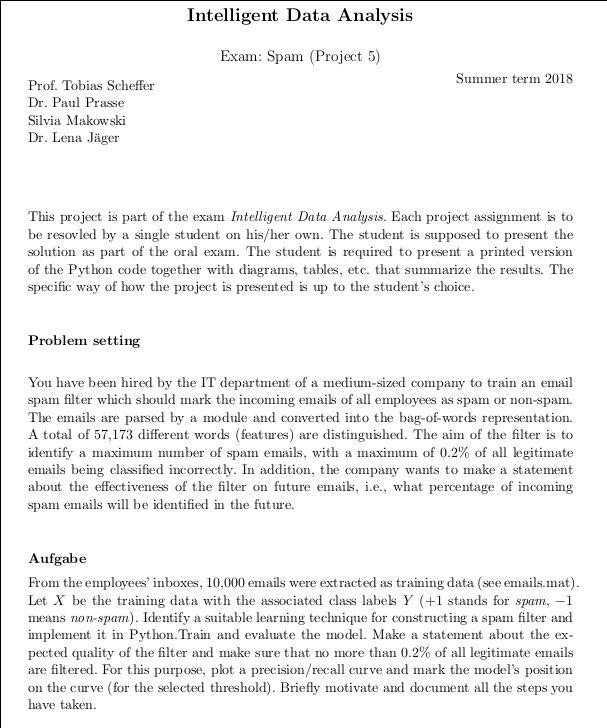
\includegraphics[trim={0.5cm 0cm 0.5cm 0.2cm},clip,width=4.7cm]{project_description.png}
					\caption{Spam project description}
				\end{figure}
				\column{0.60\linewidth}
				\begin{itemize}
					\setlength\itemsep{1.5em}
					\item Project description proposes using data in ``emails.mat" file with 10k instances and $\sim$50k features
					\item Bag-of-words form of data, which would only work for non-sequential learning
					\item Enron-spam pre-processed text data derived from Enron Corporation scandal; subset of employees' emails became publicly available \parencite{metsis2006spam}
					\item Consists of 33,716 text-based emails; 16,545 ``ham" and 17,171 spam instances
				\end{itemize}
			\end{columns}
		\end{frame}
	\end{framefont}
	
	\subsection{}
	\begin{framefont}{\footnotesize}
		\begin{frame}
			\frametitle{Objectives}
			\begin{itemize}
				\setlength\itemsep{1.5em}
				\item Utilize enron-spam emails database to implement both sequential and non-sequential supervised classifiers
				\item Meet project requirement to develop a classifier that attains 99.8\% recall on ``ham" emails
				\item Provide input into recall values for future spam emails given selected optimal threshold
				\item Additionally, provide insights into effectivity and robustness of sequential and non-sequential models
			\end{itemize}
		\end{frame}
	\end{framefont}
	
	\section{Methodologies}
	\begin{framefont}{\footnotesize}
		\begin{frame}
			\frametitle{Overview}
			\vspace{-10pt}
			\begin{columns}
				\column{0.003\linewidth}
				\column{0.40\linewidth}
				\centering
				\begin{figure}
					\captionsetup{justification=centering}
					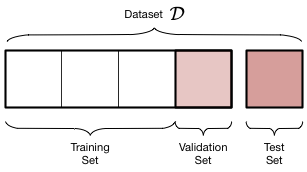
\includegraphics[width=4.3cm]{train-validate-test.png}
					\caption{Data splitting schematic \parencite{split}}
				\end{figure}
				\column{0.60\linewidth}
				\begin{itemize}
					\setlength\itemsep{1.5em}
					\item Non-sequential model: Support Vector Machine (SVM)
					\item Sequential model: CNN-LSTM with word/character embeddings
					\item Due to time limitations, K-fold cross-validation was omitted
					\item Compromise: train/validate/test on the same subsets of data for fair comparison
					\item (Train $\cup$ Validation):Test $\Longrightarrow$ 70:30
					\item Train:Validation $\Longrightarrow$ 85:15	
			\end{itemize}
			\end{columns}
		\end{frame}
	\end{framefont}
	
\begin{framefont}{\footnotesize}
	\begin{frame}
		\frametitle{Non-Sequential Model: Support Vector Machine (SVM)}
		\vspace{-10pt}
		\begin{columns}
			\column{0.003\linewidth}
			\column{0.40\linewidth}
			\centering
			\begin{figure}
				\captionsetup{justification=centering}
				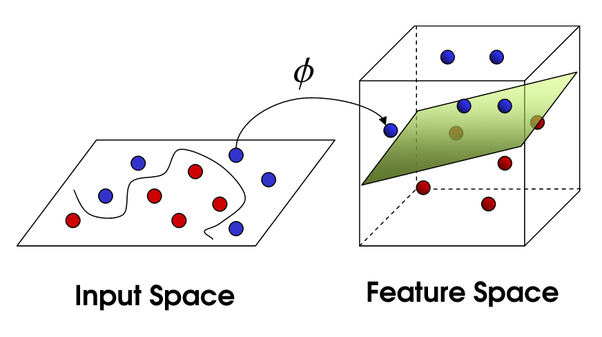
\includegraphics[width=4.3cm]{svm.png}
				\caption{Support Vector Machine (SVM) schematic \parencite{svmSchematic}}
			\end{figure}
			\column{0.60\linewidth}
			\begin{itemize}
				\setlength\itemsep{1.5em}
				\item Pre-processing text to normalized bag-of-words representation with $|V| = 5,000$ words
				\item Sklearn's \texttt{SGDClassifier} with Mini-Batch SGD and early stopping
				\item Linear and approximated RBF Kernel \texttt{(RBFSampler)}
				\item Grid-search over batch-size, regularization term $\alpha$, RBF kernel $\gamma$, and number of sampling components for \texttt{RBFSampler}
			\end{itemize}
		\end{columns}
	\end{frame}
\end{framefont}

\begin{framefont}{\footnotesize}
	\begin{frame}
		\frametitle{Sequential Model: CNN-LSTM (Words)}
		\vspace{-10pt}
		\begin{columns}
			\column{0.003\linewidth}
			\column{0.40\linewidth}
			\centering
			\begin{figure}
				\captionsetup{justification=centering}
				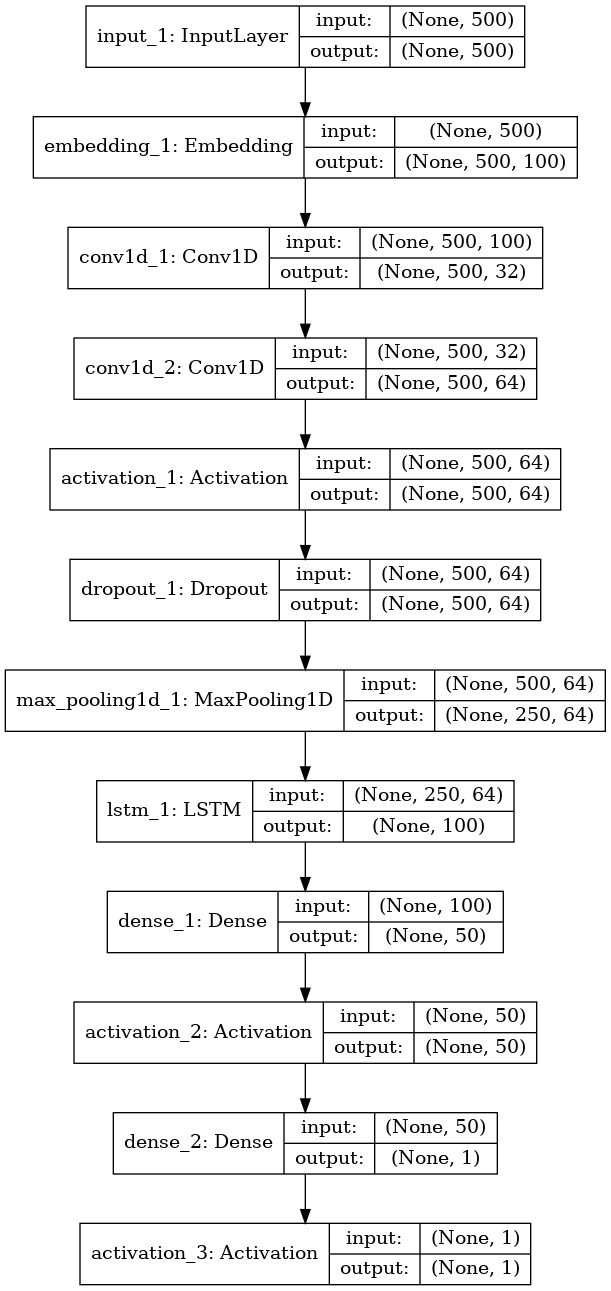
\includegraphics[width=3cm]{model.png}
				\caption{Keras schematic for CNN-LSTM (Words)}
			\end{figure}
			\column{0.60\linewidth}
			\begin{itemize}
				\setlength\itemsep{1.5em}
				\item Pre-processing text to padded/clipped integer encoded tokens with $|V| = 5,000$ words
				\item 1-dimensional CNN with varying filters to enrich sequential features; LSTM cell to capture short and long-term sequential relationships; dropout regularization for model robustness
				\item Grid-search over embedding dimensions, dropout rate, batch-size and learning rate
				\item Learning both with and without pre-trained GloVe word vectors ($\sim$6 billion tokens)
			\end{itemize}
		\end{columns}
	\end{frame}
\end{framefont}

\begin{framefont}{\footnotesize}
	\begin{frame}
		\frametitle{Sequential Model: CNN-LSTM (Words+Characters)}
		\vspace{-10pt}
		\begin{columns}
			\column{0.003\linewidth}
			\column{0.40\linewidth}
			\centering
			\begin{figure}
				\captionsetup{justification=centering}
				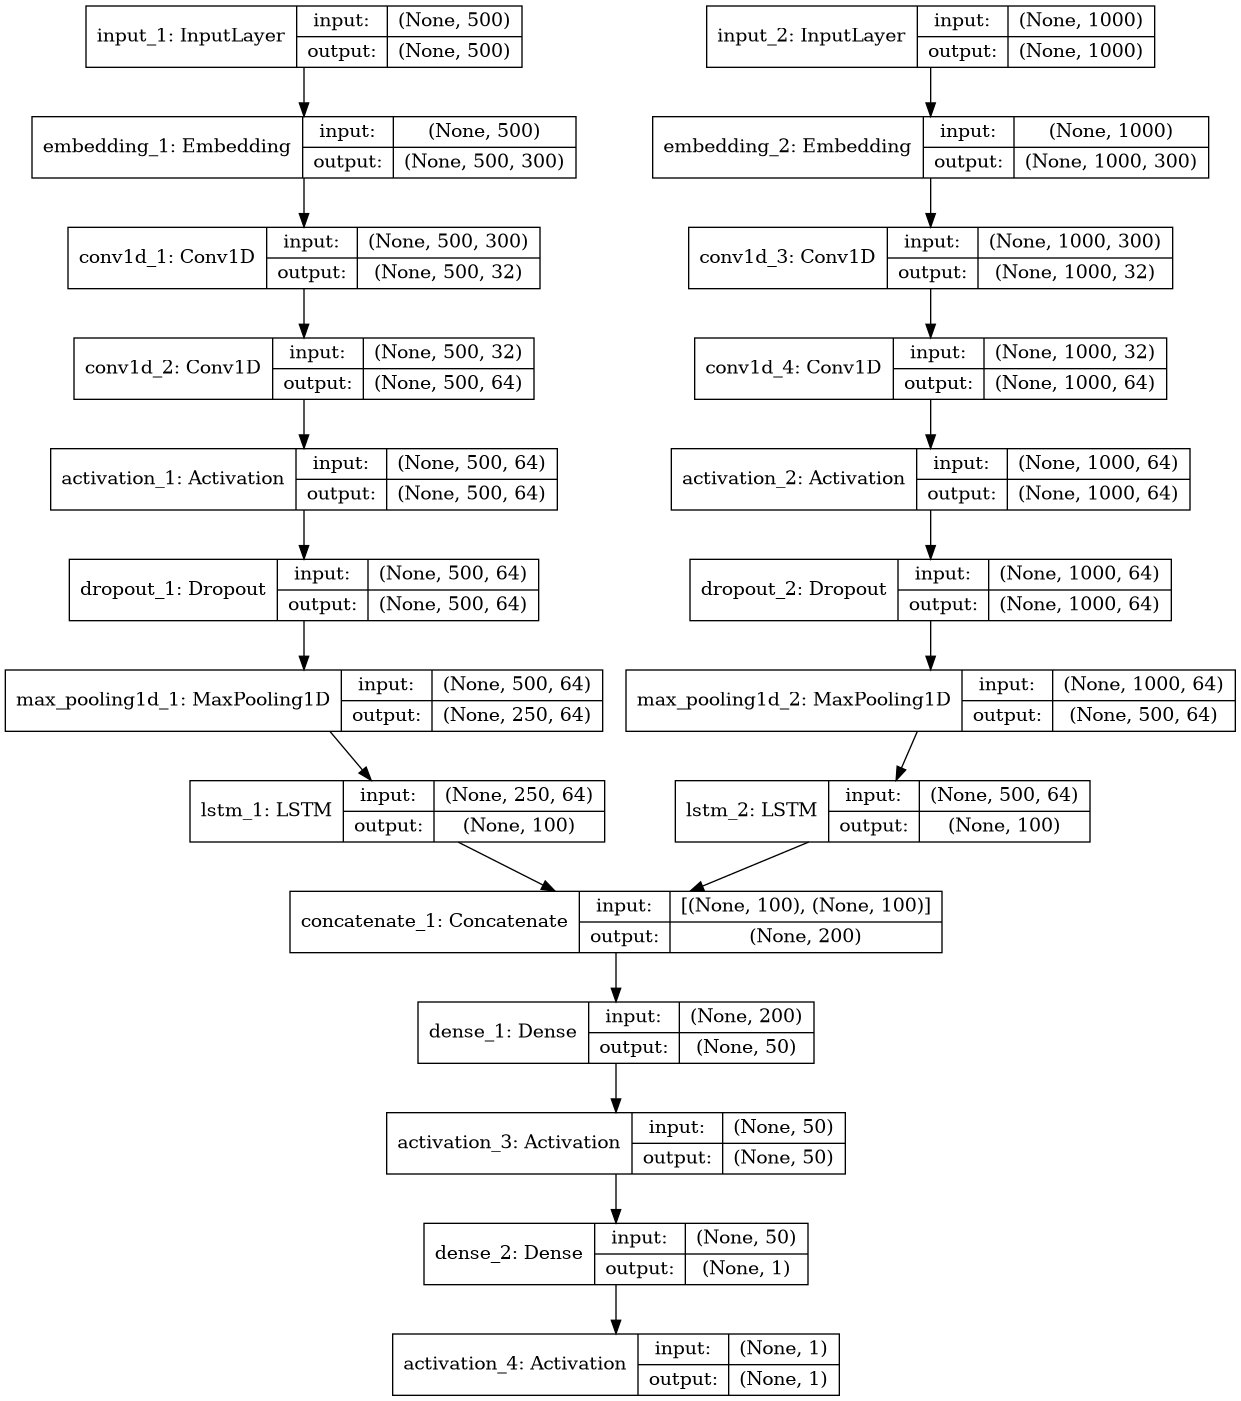
\includegraphics[width=4.6cm]{model_combined.png}
				\caption{Keras schematic for CNN-LSTM (Words+Characters)}
			\end{figure}
			\column{0.60\linewidth}
			\begin{itemize}
				\setlength\itemsep{1.5em}
				\item Using character sequences to overcome unknown token issue; same general architecture as before
				\item Grid-search over embedding dimensions, dropout rate, batch-size and learning rate
				\item Learning both with and without pre-trained GloVe word vectors ($\sim$6 billion tokens)
				\item Approximating GloVe character embeddings by averaging over character-containing word vectors \parencite{charEmbed}
			\end{itemize}
		\end{columns}
	\end{frame}
\end{framefont}

\section{Results}
\subsection{}
\begin{framefont}{\footnotesize}
	\begin{frame}
		\frametitle{Grid-search optimal models}
		\begin{table}
			\centering
			\bgroup
			\def\arraystretch{1.5}
			\begin{tabular}{|c|c|c|c|} \hline
				Classifier & Training F$_1$ & Validation F$_1$ & Test F$_1$  \\ \hhline{|=|=|=|=|}
				SVM (Linear Kernel) & 0.9880 & 0.9820 & \textbf{0.9836} \\ \hline
				SVM (Approximated RBF Kernel) & 0.4353 & 0.3494 & 0.3437 \\ \hline
				CNN-LSTM (Words) & 0.9904 & 0.9791 & 0.9753\\ \hline
				CNN-LSTM (Words+Characters) & 0.9934  & 0.9841 &  0.9808\\ \hline
				\makecell{CNN-LSTM \\(Words+GloVe)} & 0.9998  & 0.9903 & \textbf{0.9902} \\ \hline 
				\makecell{CNN-LSTM \\(Words+Characters+GloVe)} & 0.9992 & 0.9909 & \textbf{0.9902} \\ \hline
			\end{tabular}
			\egroup
			\caption{Summary of grid-search optimal models; zero rule classifier baseline is 50.9\%}
		\end{table}
		\begin{itemize}
			\item Both sequential and non-sequential models achieve high F$_1$ test scores
		\end{itemize}
	\end{frame}
\end{framefont}

\subsection{}
\begin{framefont}{\footnotesize}
	\begin{frame}
		\frametitle{``Ham" Relative Importance Analysis (SVM)}
		\centering
		\begin{figure}
			\captionsetup{justification=centering}
			\includegraphics[width=10.5cm]{ham_words.pdf}
			\caption{Relative importance analysis for SVM (linear kernel)}
		\end{figure}
	\end{frame}
\end{framefont}

\subsection{}
\begin{framefont}{\footnotesize}
	\begin{frame}
		\frametitle{Spam Relative Importance Analysis (SVM)}
		\centering
		\begin{figure}
			\captionsetup{justification=centering}
			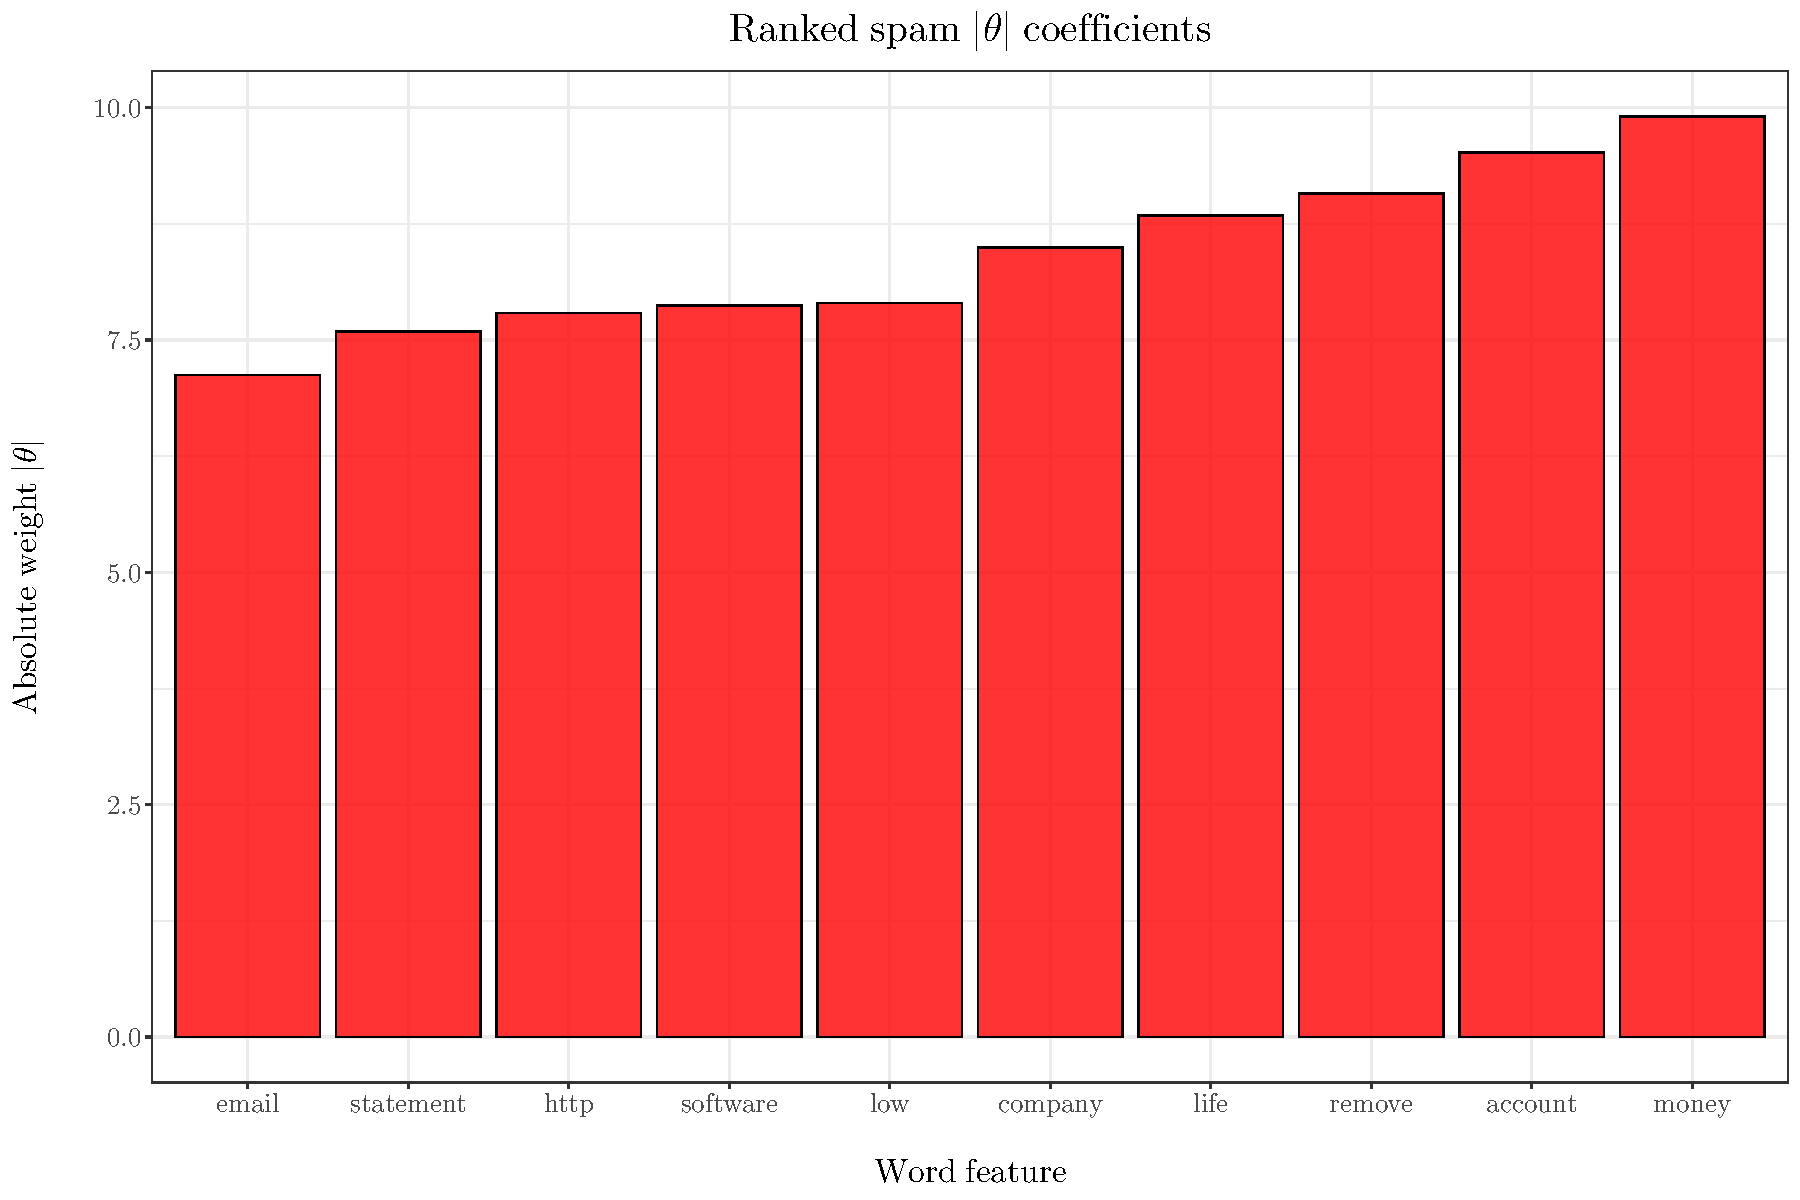
\includegraphics[width=10.5cm]{spam_words.pdf}
			\caption{Relative importance analysis for SVM (linear kernel)}
		\end{figure}
	\end{frame}
\end{framefont}

\section{Evaluation}
\subsection{}
\begin{framefont}{\footnotesize}
	\begin{frame}
		\frametitle{Optimal Threshold Analysis}
		\centering
		\begin{figure}
			\captionsetup{justification=centering}
			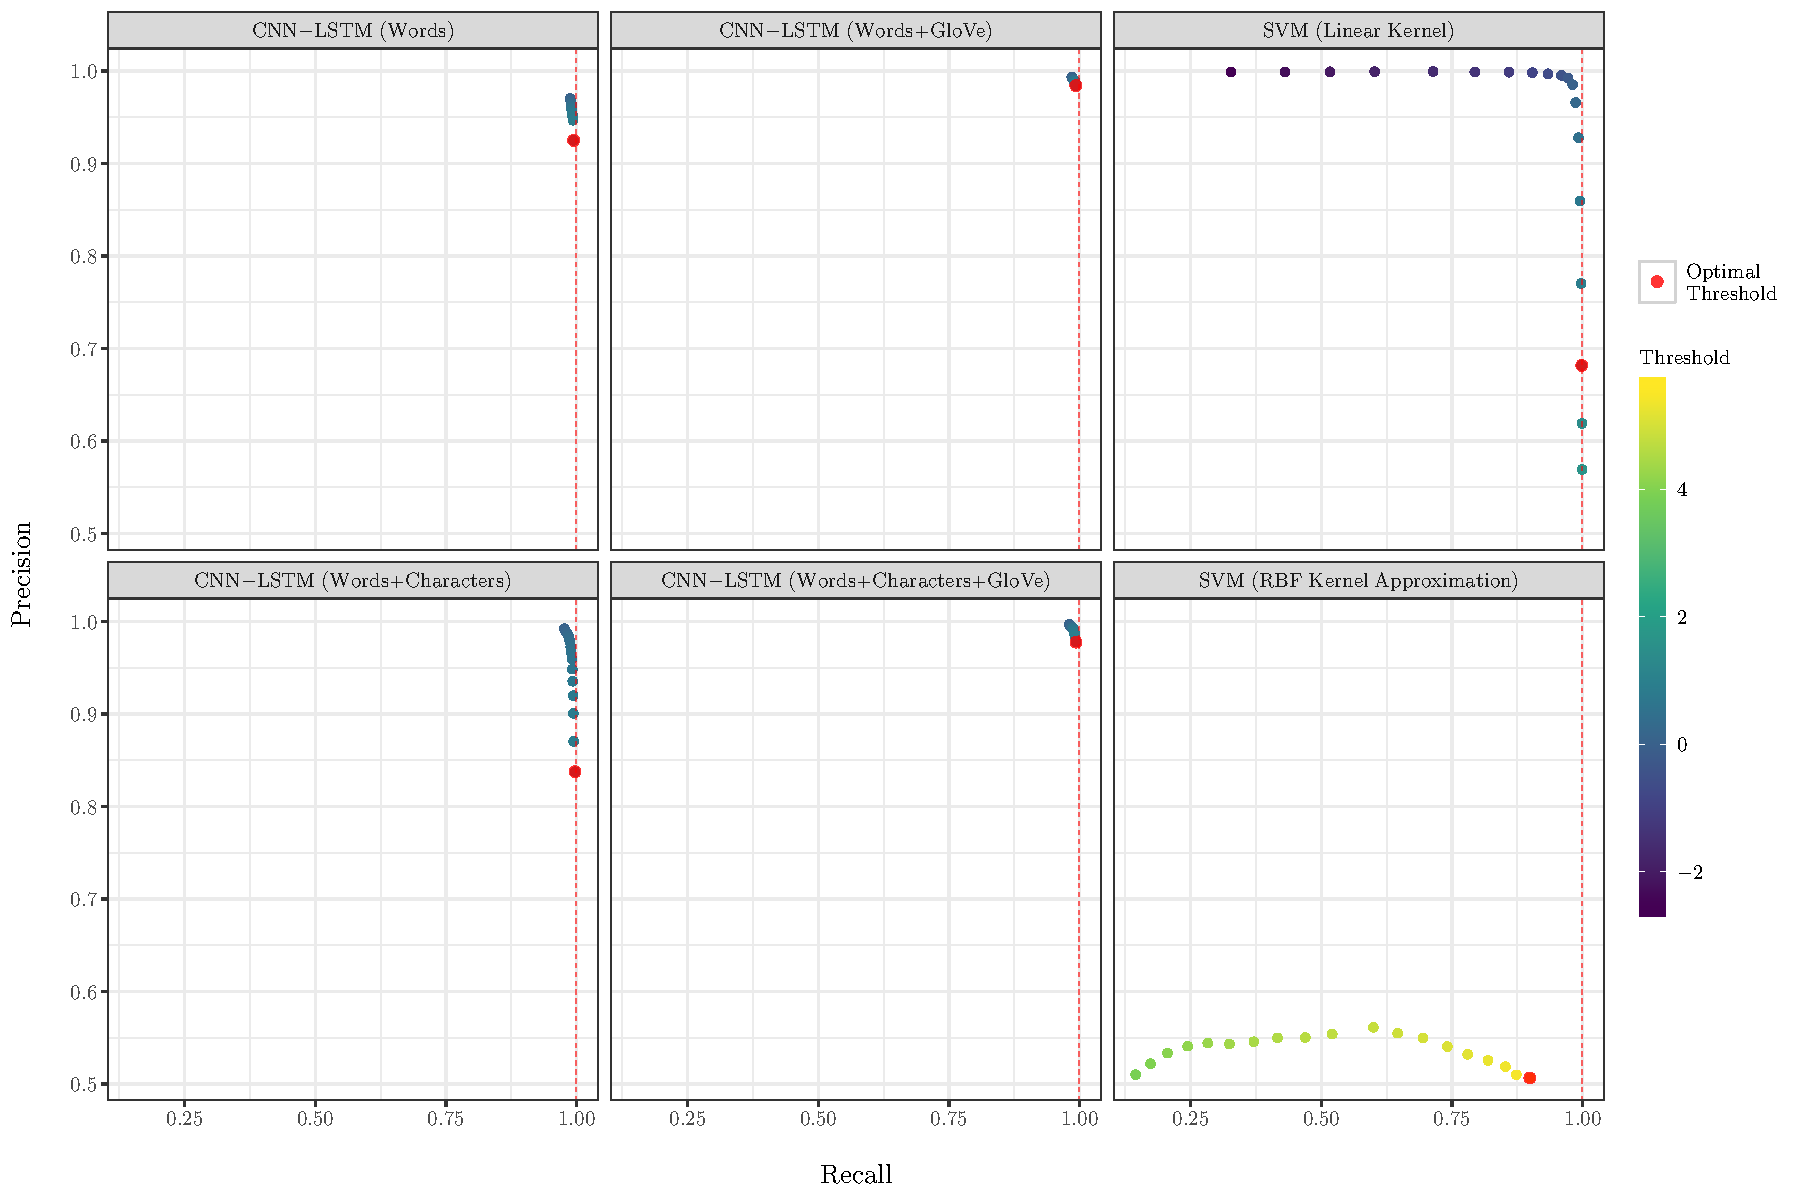
\includegraphics[trim={0cm 0cm 0.2cm 0cm},clip,width=11.2cm]{combined.pdf}
			\caption{Precision-Recall curve (ham label) for optimal threshold analysis}
		\end{figure}
	\end{frame}
\end{framefont}

\subsection{}
\begin{framefont}{\footnotesize}
	\begin{frame}
		\frametitle{Optimal Threshold Performance}
		\begin{table}
			\centering
			\bgroup
			\def\arraystretch{1.5}
			\begin{tabular}{|c|c|c|c|} \hline
				Classifier & Threshold & Recall (Spam) & Recall (Ham) \\ \hhline{|=|=|=|=|}
				SVM (Linear Kernel) & 1.171 & \color{red} 0.5509 & \textbf{0.9982} \\ \hline
				SVM (Approximated RBF Kernel) & 5.552 & 0.1558 & 0.8991 \\ \hline
				CNN-LSTM (Words) & 0.9444 & 0.9224 & 0.9943 \\ \hline
				CNN-LSTM (Words+Characters) & 0.9444  & \color{red} 0.8137 &  \textbf{0.9971} \\ \hline
				\makecell{CNN-LSTM \\(Words+GloVe)} & 0.9444  & \color{ao(english)} 0.9846  & \textbf{0.9929} \\ \hline
				\makecell{CNN-LSTM \\(Words+Characters+GloVe)} & 0.9444 & \color{ao(english)} 0.9781 & \textbf{0.9930} \\ \hline
			\end{tabular}
			\egroup
			\caption{Results of optimal threshold analysis}
		\end{table}
		\begin{itemize}
			\item Trade off between ham and spam recall; either accept low recall for spam or compromise with lower recall for ham
		\end{itemize}
	\end{frame}
\end{framefont}

\subsection{}
\begin{framefont}{\footnotesize}
	\begin{frame}
		\frametitle{Blind Dataset Performance (SMS Spam)}
		\begin{table}
			\centering
			\bgroup
			\def\arraystretch{1.5}
			\begin{tabular}{|c|c|} \hline
				Classifier & Blind F$_1$ \\ \hhline{|=|=|}
				SVM (Linear Kernel) & \textbf{0.4688}  \\ \hline
				SVM (Approximated RBF Kernel) & 0.1785 \\ \hline
				CNN-LSTM (Words) & \textbf{0.5090} \\ \hline
				CNN-LSTM (Words+Characters) & 0.4416 \\ \hline
				\makecell{CNN-LSTM \\(Words+GloVe)} & 0.2913  \\ \hline
				\makecell{CNN-LSTM \\(Words+Characters+GloVe)} & 0.3017  \\ \hline
			\end{tabular}
			\egroup
			\caption{Results of blind data test; zero rule classifier obtains 87\% due to class imbalance}
		\end{table}
		\vspace{-10pt}
		\begin{itemize}
			\item Words-based models perform best on blind dataset (albeit worse than zero rule classifier)
			\item Considering sequential nature of data contributes to some robustness
		\end{itemize}
	\end{frame}
\end{framefont}

\section{Conclusions}
\subsection{}
\begin{framefont}{\footnotesize}
	\begin{frame}
		\frametitle{Conclusions}
		\begin{itemize}
			\setlength\itemsep{1.2em}
			\item For spam detection, both sequential and non-sequential models are effective
			\item Trade-off exists between ``ham" and spam recall; an informed decision must be made
			\item Both words-based sequential and non-sequential models tend to be robust to new datasets; although sequential models tend to carry richer and more discriminating features
			\item High cost of training CNN-LSTM; perhaps not economical for a company to deploy GPU on IMAP server
			\item \textbf{SVM would be a more efficient and scalable option}
		\end{itemize}
	\end{frame}
\end{framefont}

\subsection{}
\begin{framefont}{\footnotesize}
	\begin{frame}
		\frametitle{Improvements to Embeddings in CNN-LSTM}
		\vspace{-10pt}
		\begin{columns}
			\column{0.003\linewidth}
			\column{0.40\linewidth}
			\centering
			\begin{figure}
				\captionsetup{justification=centering}
				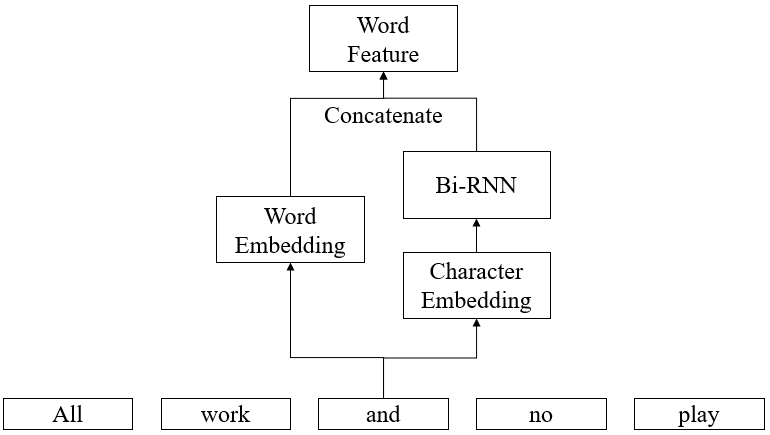
\includegraphics[width=4.5cm]{improved_rnn.png}
				\caption{Improved word-character embedding model \parencite{improvedRNN}}
			\end{figure}
			\column{0.60\linewidth}
			\begin{itemize}
				\setlength\itemsep{1.5em}
				\item Separate pipeline for character sequences leads to symbolic overfitting on types of datasets
				\item Can overcome unknown tokens but contributes uncertainty in terms of dialects and expressions
				\item \textcite{improvedRNN} proposes a bidirectional LSTM to enrich word vector features
				\item This could address the unknown token issue without leading to overfitting on entire character sequences
			\end{itemize}
		\end{columns}
	\end{frame}
\end{framefont}


% blind dataset with SMS set
% much shorter and different type of ham
% character analysis not useful as it adapts to general writing style and might be robust to shorter and quick writing styles
% character analysis overfits to company's email writing style
% glove embeddings perform worse as they are trained on proper English language usage, but SMS spam datasest has many slangs
% words-based-models perform well since some or many legitimate words are still present
% sequential analysis still provides an additional edge

% make some hypotheses here, advantages and limitations
% highlight why LSTM without glove embeddings succeeds
% highlight why SVM also performs well
% conclude that sequential information is important and makes models more robust
% might not be most practical for spam since IMAP servers may not have GPUs to use RNNs
% SVMs might be a good alternative
% fill up blbliography with some relevant articles

% add animations/transitions

%# schema:
% plot threshold values on PR curve with orientation on non-spam class to select best model, to answer qn. 1, plot PR curves with F1-contour lines
% create classification reports for best thresholds, to answer qn. 2 (combined plot)
% 1st table with basic F1 performance, then charts with thresholds, then combined confusion matrices
% then table with adjust thresholds, precision on non-spam, recall on spam and overall F1 performance
% lastly table with blind dataset and F1 performances to find most robust models
% make nice tables, think of how to present uniform classifier
% replace with better quality images, add training and validation f1 scores

%# extra:
% add charts and more structured information on github, with separate docs on function implementation
% make more structured data download systems, with dialogue oriented approach
% figure out R command line parsing methods

\begin{frame}[allowframebreaks]
	\frametitle{Bibliography}
	\nocite{*}
	\printbibliography[title = {Bibliography}]
\end{frame}

\end{document}

%	\section{Methodologies}
%\subsection{}
%\begin{frame}
%	\frametitle{Rational Speech Act: Literal vs. Pragmatic Speaker}
%	\begin{figure}
%		\begin{tikzpicture}
%		\node[anchor=south west,inner sep=0] (image) at (0,0) {\includegraphics[trim={5cm 5cm 4.6cm 0cm},clip,width=8cm]{rational.png}};
%		\uncover<2-5>{\draw[red,thick,dashed] (5.75,0) rectangle (8.25,2.5);}
%		\end{tikzpicture}
%		\vspace{5pt}
%		\captionsetup{justification=centering}
%		\caption{Example to show pragmatic speaker behavior \parencite{frank_2016}}
%	\end{figure}
%	\vspace{-5pt}
%	\begin{itemize}
%		\setlength\itemsep{1em}
%		\item<3-> Literal speaker: $\{$Face, glasses, hat$\}$
%		\item<4-> Pragmatic speaker: $\{$Hat$\}$
%		\item<5> Pragmatic speaker would identify object by minimizing redundancy or maximizing \textit{utility}
%	\end{itemize}
%\end{frame}
%
%\subsection{}
%\begin{frame}
%	\frametitle{Rational Speech Act: Literal vs. Pragmatic Listener}
%	\begin{figure}
%		\begin{tikzpicture}
%		\node[anchor=south west,inner sep=0] (image) at (0,0) {\includegraphics[width=8cm]{objects.png}};
%		\uncover<3-4>{\draw[red,thick,dashed] (0.5,0) rectangle (5.1,2.5);}
%		\end{tikzpicture}
%		\vspace{5pt}
%		\captionsetup{justification=centering}
%		\caption{Example to highlight difference between literal and pragmatic listener \parencite{scontras_2016}}
%	\end{figure}
%	\vspace{-10pt}
%	\begin{itemize}
%		\setlength\itemsep{1em}
%		\item<2-> Assume given cue to be $\{$Blue$\}$
%		\item<3-> Literal listener: $\{$Square, Blue$\}$ $\lor$ $\{$Circle, Blue$\}$
%		\item<4-> Pragmatic listener: $\{$Square, Blue$\}$ $\longrightarrow$ \textbf{why?}
%	\end{itemize}
%\end{frame}
%
%\subsection{}
%\begin{frame}
%	\frametitle{Rational Speech Act: Recursion}
%	\begin{figure}
%		\includegraphics[width=8cm]{recursive.png}
%		\captionsetup{justification=centering}
%		\caption{Recursive process of communication between listener and speaker \parencite{yung2016modelling}}
%	\end{figure}
%	\vspace{-10pt}
%	\begin{itemize}
%		\setlength\itemsep{1em}
%		\item<1-> Communication between listener $L_n$ and speaker $S_n$ is theoretically recursive
%		\item<2> In practice, the recursion is usually cut-off at $L_2$
%	\end{itemize}
%\end{frame}
%
%\subsection{}
%\begin{frame}
%	\frametitle{Rational Speech Act: Theoretical Functions}
%	\begin{figure}
%		\includegraphics[width=9cm]{eqns.png}
%		\captionsetup{justification=centering}
%		\caption{Functions for calculating probabilities at recursive stages \parencite{scontras_2016}}
%	\end{figure}
%	\vspace{-10pt}
%	\begin{itemize}
%		\setlength\itemsep{1em}
%		\item These equations form the basic framework of the Rational Speed Act, albeit specifically cut-off at $L_1$
%		\item Utility function: $U_{S_1}(u;s) = \ln(L_0(s|u)) - C(u)$
%	\end{itemize}
%\end{frame}
%
%\subsection{}
%\begin{framefont}{\footnotesize}
%	\begin{frame}
%		\frametitle{Rational Speech Act: Application to Discourse}
%		\begin{columns}
%			\column{0.38\linewidth}
%			\begin{flalign*}
%			& 1. ~~s_i = \argmax_{s \in S} P_L(s|d,C)\label{eq:1}\\[2pt]
%			& 2. ~~P_{L_0}(s|d,C) = \dfrac{count(s,d,C)}{count(d,C)}\\[2pt]
%			& 3. ~~P_L(s) = \dfrac{count(s)}{\sum_{s' \in S}count(s')}\\[10pt]
%			& 4. ~~P_{S_n}(d|s,C) \\[2pt]
%			& = \dfrac{\exp(\ln P_{L_{n-1}}(s|d,C)-cost(d))}{\sum_{d' \in D}\exp(\ln P_{L_{n-1}}(s|d',C)-cost(d'))}\\[10pt]
%			& 5. ~~P_{L_n}(s|d,C) \\[2pt]
%			&= \dfrac{P_{S_n}(d|s,C)P_L(s)}{\sum_{s' \in S} P_{S_n}(d|s',C)P_L(s')}
%			\end{flalign*}
%			\column{0.38\linewidth}
%			\begin{itemize}
%				\setlength\itemsep{1.5em}
%				\item<2-> $d$: discourse connectives in PDTB
%				\item<3-> $s$: sense; 15 sense labels
%				\item<4-> $C$: context; sense and/or form of the directly preceding discourse connective
%				\item<5-> $cost(d)$: cost of discourse connective $d$; 
%				tuned to positive value for explicit and $0$ for implicit
%			\end{itemize}
%		\end{columns}
%	\end{frame}
%\end{framefont}
%
%\section{Results and Evaluation}
%\subsection{}
%\begin{framefont}{\footnotesize}
%	\begin{frame}
%		\frametitle{Internal Parser Performance}
%		\vspace{-10pt}
%		\begin{columns}
%			\column{0.45\linewidth}
%			\centering
%			\begin{figure}
%				\captionsetup{justification=centering}
%				\includegraphics[width=4.8cm]{internal.png}
%				\caption{Improvement of internal performance given pragmatic listener/speaker assumptions \parencite{yung2016modelling}}
%			\end{figure}
%			\column{0.50\linewidth}
%			\begin{itemize}
%				\setlength\itemsep{1em}
%				\item Training: Sections 2-22 of PDTB
%				\item Testing: Sections 0, 1, 23 and 24 of PDTB
%				\item Internal testing of literal listener vs. pragmatic listener showed improvement in accuracy above baseline
%				\item Accuracies cap off at $L_1$, meaning pragmatic listener is unlikely to emulate deeper discourse productions of speaker
%			\end{itemize}
%		\end{columns}
%	\end{frame}
%\end{framefont}
%
%\subsection{}
%\begin{framefont}{\footnotesize}
%	\begin{frame}
%		\frametitle{External Parser Performance}
%		\vspace{-10pt}
%		\begin{columns}
%			\column{0.005\linewidth}
%			\column{0.45\linewidth}
%			\centering
%			\begin{figure}
%				\captionsetup{justification=centering}
%				\includegraphics[width=4.8cm]{external.png}
%				\caption{Improvement of external performance given pragmatic listener/speaker assumptions \parencite{yung2016modelling}}
%			\end{figure}
%			\column{0.55\linewidth}
%			\begin{itemize}
%				\setlength\itemsep{1em}
%				\item Comparison with output of CONLL shared task winning parser \parencite{wang2015refined}
%				\item Output of winning parser is used to replace $P_L(s)$ in pragmatic listener probability distribution
%				\item $P'_{L_1} =\dfrac{P_{S_1}(d|s,C)P_{parser}(s)}{\sum_{s' \in S} P_{S_1}(d|s',C)P_{parser}(s')}$
%				\item Resulting F-1 scores improve with pragmatic generalization
%			\end{itemize}
%		\end{columns}
%	\end{frame}
%\end{framefont}
%
%\section{Discussion}
%\subsection{}
%\begin{frame}
%	\frametitle{Discussion}
%	\begin{itemize}
%		\setlength\itemsep{1.5em}
%		\item Interesting article because it incorporates psycholinguistic perspective into discourse connective interpretation
%		\item<2,5-> $cost(d)$ could be refined for both explicit and implicit DCs based on other stress parameters
%		\item<3,5-> The context $C$ of a discourse relation could be refined to include longer-distance parameters
%		\item<4,5-> Does the rational speaker/listener assumption hold in all contexts?
%	\end{itemize}
%\end{frame}